\chapter{Esperimenti di simulazione}\label{chp:esperimenti-simulazione}
In accordo agli obiettivi dello studio, per la progettazione degli esperimenti di simulazione, è stata considerata unicamente l'analisi dello stato transiente del sistema. Infatti, perderebbe di significato considerare lo stato stazionario per determinare il numero minimo di serventi necessari affinché vengano soddisfatti i QoS descritti nel capitolo \ref{chp:obiettivi}. Questo perché in una giornata lavorativa il sistema non riesce a raggiungere lo stato stazionario prima che si verifichi la condizione di scarico (\textit{"close the door"}) ed inoltre rimane forte l'influenza delle condizioni iniziali. 

Per completezza, nella sezione \ref{sec:esperimenti-simulazione-stazionario}, è mostrato il mancato raggiungimento della stazionarietà, nell'arco di una giornata lavorativa, da parte del sistema. 

\section{Progetto degli esperimenti}\label{sec:esperimenti-simulazione-1}
Per realizzare l'analisi transiente del sistema è stata adottata la tecnica \textit{replication}, dove:
\begin{itemize}
\item Il numero di repliche adottato nella simulazione è pari a \texttt{10000}, scelto con l'obiettivo di perdere la dipendenza dal seme iniziale.
\item Il seme iniziale adottato è \texttt{9}, settato unicamente ad inizio simulazione al fine di evitare di generare più volte le stesse sequenze di variate pseudocasuali. Infatti, se si scegliesse manualmente il seed di ciascuna replica, potrebbe verificarsi un overlap nella generazione.
\item \texttt{START = 0} e \texttt{STOP = 480} come descritto in sezione \ref{sec:modello-computazionale-clock}.
\end{itemize}

Inoltre:
\begin{itemize}
\item È stato utilizzato il programma \texttt{estimate} per il calcolo delle realizzazioni degli intervalli di confidenza al 95\%.
\item È stato utilizzato il programma \texttt{uvs} per il calcolo di media e deviazione standard.
\end{itemize}

Di seguito sono riportate le descrizioni degli esperimenti di simulazione compiuti, per ciascuno dei quali è stata adottata la tecnica \textit{replication} appena illustrata.

\subsection*{Numero minimo di sportelli}
Per individuare il numero minimo $M^*$ di sportelli da mantenere operativi in una giornata lavorativa, al fine di soddisfare i QoS (cap. \ref{chp:obiettivi}), un primo esperimento condotto è stato quello di analizzare l'attesa media di ciascuna classe d'utenza al variare di $M$.

A tal proposito, è stato simulato il sistema per un'intera giornata di lavoro, assumendo che i clienti iniziassero ad arrivare all'ufficio postale solo successivamente all'apertura (sistema inizialmente scarico).

\subsection*{Andamento dell'attesa nell'arco della giornata}
Una volta individuato il valore $M^*$, è stata studiata l'evoluzione dell'attesa media per ciascuna classe d'utenza all'avanzare del tempo di simulazione.

Per realizzare quest'esperimento è stata eseguita una campionatura oraria delle statistiche, ovvero sono state effettuate:
\begin{itemize}
\item 10000 repliche in cui il campionamento avviene al $60$-esimo minuto di simulazione
\item 10000 repliche in cui il campionamento avviene al $120$-esimo minuto di simulazione
\item $\dots$
\item 10000 repliche in cui il campionamento avviene al $480$-esimo minuto di simulazione
\end{itemize}
dove la procedura utilizzata per inferire le statistiche è quella illustrata nel capitolo \ref{sec:modello-computazionale-campionamento-stat}.
	
\section{Esecuzione degli esperimenti ed analisi degli output}
\subsection*{Numero minimo di sportelli}
I risultati dell'esperimento condotto sono riportati sia in forma tabellare (tab. \ref{table:esperimenti-simulazione-1}) che in forma grafica (fig. \ref{fig:esperimenti-simulazione-1}).

È immediato osservare che per rispettare i requisiti di qualità stabiliti nel capitolo \ref{chp:obiettivi}, mostrati nei grafici tramite linee rosse tratteggiate, il numero minimo di serventi è $M^* = 4$. Infatti, dalla figura \ref{fig:esperimenti-simulazione-1d} si evince che con $M = 3$ non è possibile rispettare il QoS (in tabella \ref{table:esperimenti-simulazione-1b} è evidenziato in {\color{red}rosso} il valore di  attesa che lo supera).

\subsection*{Andamento dell'attesa nell'arco della giornata}
I risultati dell'esperimento condotto sono riportati sia in forma tabellare (tab. \ref{table:esperimenti-simulazione-2}) che in forma grafica (figg. \ref{fig:esperimenti-simulazione-2} e \ref{fig:esperimenti-simulazione-3}).

In particolare:
\begin{itemize}
\item In figura \ref{fig:esperimenti-simulazione-2} è possibile osservare come per tutte le classi d'utenza, dopo circa 5 ore dall'apertura del centro postale, l'attesa media si stabilizza intorno al valore medio calcolato sull'intera giornata lavorativa, di durata non inferiore a 480 minuti (istante in cui si interrompe l'erogazione dei ticket).
\item In figura \ref{fig:esperimenti-simulazione-3} è possibile osservare come:
\begin{itemize}
\item I tempi d'attesa delle classi siano maggiori al diminuire della priorità in ogni fascia oraria, a partire dalla seconda ora di servizio.
\item I tempi d'attesa per le classi \sr{} \textsl{BancoPosta} e \textsl{Standard} sono di un ordine di grandezza superiore a quelli delle restanti, perché serviti dal singolo servente dedicato piuttosto che da 4 server in parallelo.
\end{itemize}
\end{itemize}

\section{Mancato raggiungimento dello stato stazionario}\label{sec:esperimenti-simulazione-stazionario}
Per mostrare il mancato raggiungimento dello stato stazionario è stato simulato il sistema per un periodo superiore ad una giornata lavorativa ($960$ minuti di erogazione dei ticket). 

In figura \ref{fig:esperimenti-simulazione-4} e in tabella \ref{table:esperimenti-simulazione-3} è mostrato come il tempo medio d'attesa per la classe \uo{} \textsl{Standard} continua a crescere dopo i primi $480$ minuti (tempo di erogazione dei ticket in una normale giornata lavorativa). 

Il mancato raggiungimento della stazionarietà da parte di una classe d'utenza implica il mancato raggiungimento della stazionarietà di tutto il sistema.

Inoltre:
\begin{itemize}
\item È stata adottata la tecnica replication con lo stesso numero di repliche ($10000$) e seed iniziale ($9$) descritti in precedenza nella sezione \ref{sec:esperimenti-simulazione-1}. L'unica variazione è stata quella di impostare il parametro \texttt{STOP} pari a $960$.
\item Sono stati utilizzati i programmi \texttt{uvs} e \texttt{estimate} rispettivamente per il calcolo della media, della deviazione standard e delle realizzazioni degli intervalli di confidenza al 95\%.
\end{itemize}

\newpage
\section{Grafici e tabelle}
\subsection*{Numero minimo di sportelli}
\captionsetup[table]{justification=centering}
\begin{table}[ht]
\centering
\begin{subtable}{0.5\textwidth}
\centering
{\tablecolors
\begin{tabular}{|c|c|c|c|}
\hline
$c$ & $\bar{d}_c$ & $s_c$ & $w$\\
\hline
0 & 6.924 & 3.068 & 0.06 \\
\hline
1 & 10.064 & 6.333 & 0.12 \\
\hline
2 & 28.191 & 20.506 & 0.40 \\
\hline
3 & 141.439 & 81.084 & 1.59 \\
\hline
4 & 10.251 & 7.008 & 0.14 \\
\hline
5 & 15.865 & 8.988 & 0.18 \\
\hline
\end{tabular}}
\caption{$M = 2$}
\end{subtable}%
\begin{subtable}{0.5\textwidth}
\centering
{\tablecolors
\begin{tabular}{|c|c|c|c|}
\hline
$c$ & $\bar{d}_c$ & $s_c$ & $w$\\
\hline
0 & 2.567 & 1.594 & 0.03 \\
\hline
1 & 3.119 & 2.379 & 0.05 \\
\hline
2 & 5.619 & 4.178 & 0.08 \\
\hline
3 & {\color{red}16.162} & {\color{red}17.656} & {\color{red}0.35} \\
\hline
4 & 8.436 & 6.945 & 0.14 \\
\hline
5 & 13.029 & 9.144 & 0.18 \\
\hline
\end{tabular}}
\caption{$M = 3$}
\label{table:esperimenti-simulazione-1b}
\end{subtable}
\begin{subtable}{0.5\textwidth}
\centering
{\tablecolors
\begin{tabular}{|c|c|c|c|}
\hline
$c$ & $\bar{d}_c$ & $s_c$ & $w$\\
\hline
0 & 0.780 & 0.756 & 0.01 \\
\hline
1 & 0.881 & 1.027 & 0.02 \\
\hline
2 & 1.347 & 1.274 & 0.02 \\
\hline
3 & 2.496 & 3.126 & 0.06 \\
\hline
4 & 6.224 & 6.256 & 0.12 \\
\hline
5 & 9.451 & 8.221 & 0.16 \\
\hline
\end{tabular}}
\caption{$M = 4$}
\end{subtable}
\caption{Media ($\bar{d}_c$), deviazione standard ($s_c$) e ampiezza dell'intervallo di confidenza al 95\% ($w$) per l'attesa (espressa in minuti) di ciascuna classe d'utenza $c$, al variare di $M$}
\label{table:esperimenti-simulazione-1}
\end{table}

\captionsetup[figure]{justification=centering}
\begin{figure}[ht]
\centering
\begin{subfigure}[b]{0.475\textwidth}
\centering
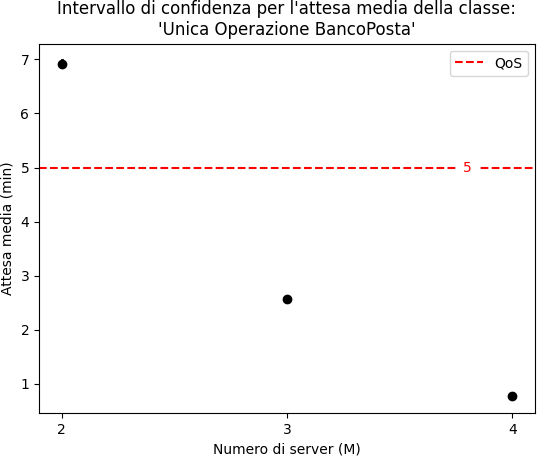
\includegraphics[width=\textwidth]{plots/d0-trans}
\caption{\uo{} \textsl{BancoPosta}}    
\end{subfigure}
\hfill    
\begin{subfigure}[b]{0.475\textwidth}  
\centering 
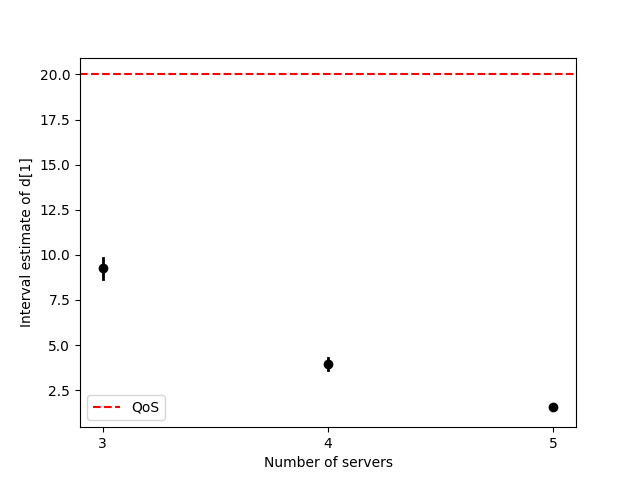
\includegraphics[width=\textwidth]{plots/d1-trans}
\caption{\pp{} \textsl{BancoPosta}}    
\end{subfigure}

\vskip\baselineskip

\begin{subfigure}[b]{0.475\textwidth}   
\centering 
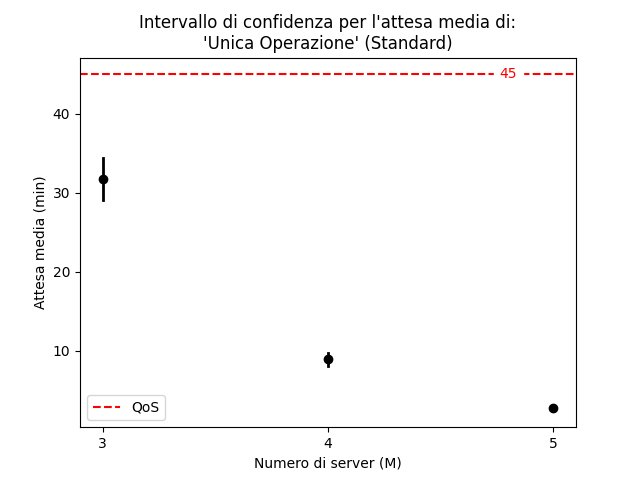
\includegraphics[width=\textwidth]{plots/d2-trans}
\caption{\uo{} \textsl{Standard}}    
\end{subfigure}
\hfill
\begin{subfigure}[b]{0.475\textwidth}   
\centering 
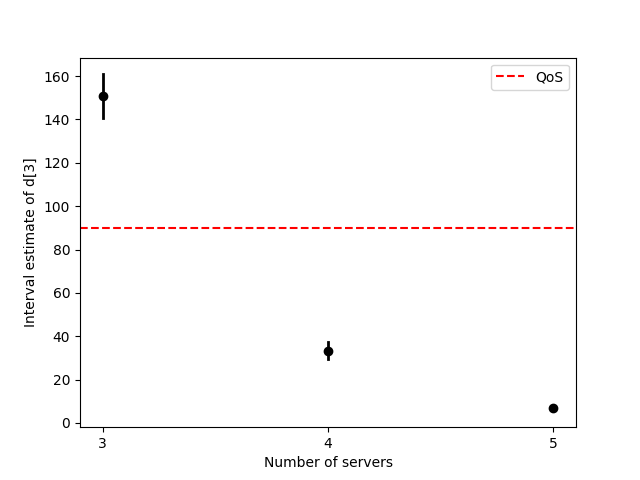
\includegraphics[width=\textwidth]{plots/d3-trans}
\caption{\pp{} \textsl{Standard}}
\label{fig:esperimenti-simulazione-1d}  
\end{subfigure}

\vskip\baselineskip

\begin{subfigure}[b]{0.475\textwidth}   
\centering 
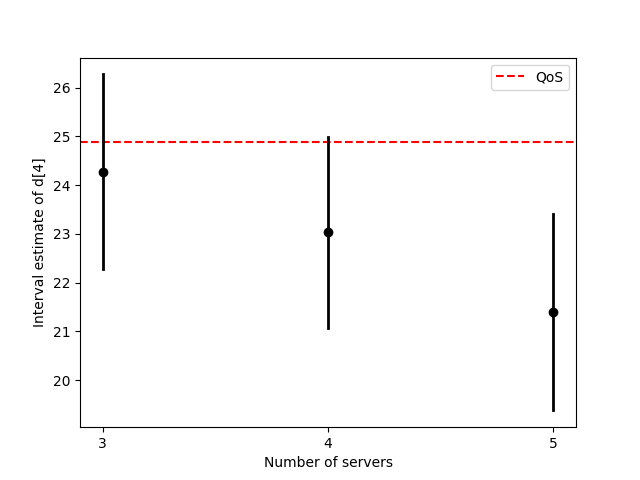
\includegraphics[width=\textwidth]{plots/d4-trans}
\caption{\sr{} \textsl{BancoPosta}}    
\end{subfigure}
\hfill
\begin{subfigure}[b]{0.475\textwidth}   
\centering 
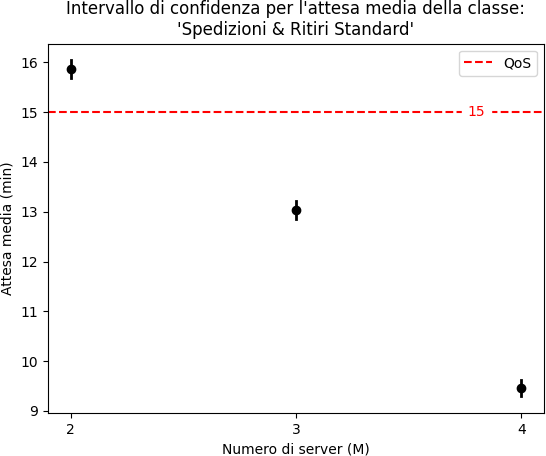
\includegraphics[width=\textwidth]{plots/d5-trans}
\caption{\sr{} \textsl{Standard}}    
\end{subfigure}
\caption{Intervalli di confidenza al 95\% per l'attesa media (espressa in minuti) di ciascuna classe d'utenza, al variare di $M$}
\label{fig:esperimenti-simulazione-1}
\end{figure}

\subsection*{Andamento dell'attesa nell'arco della giornata}
\captionsetup[table]{justification=centering}
\begin{table}[ht]
\centering
\begin{subtable}[t]{0.33\textwidth}
\centering
{\tablecolors
\begin{tabular}{|c|c|c|c|}
\hline
$t$ & $\bar{d}_0$ & $s_0$ & $w$\\
\hline
60 & 0.398 & 1.484 & 0.03 \\
\hline
120 & 0.640 & 1.494 & 0.03 \\
\hline
180 & 0.719 & 1.310 & 0.03 \\
\hline
240 & 0.745 & 1.127 & 0.02 \\
\hline
300 & 0.756 & 0.952 & 0.02 \\
\hline
360 & 0.772 & 0.876 & 0.02 \\
\hline
420 & 0.784 & 0.815 & 0.02 \\
\hline
480 & 0.795 & 0.772 & 0.02 \\
\hline
\end{tabular}}
\caption{\uo{} \textsl{BancoPosta}}
\end{subtable}%
\begin{subtable}[t]{0.33\textwidth}
\centering
{\tablecolors
\begin{tabular}{|c|c|c|c|}
\hline
$t$ & $\bar{d}_1$ & $s_1$ & $w$\\
\hline
60 & 0.331 & 1.534 & 0.03 \\
\hline
120 & 0.676 & 2.239 & 0.04 \\
\hline
180 & 0.795 & 1.862 & 0.04 \\
\hline
240 & 0.833 & 1.484 & 0.03 \\
\hline
300 & 0.860 & 1.336 & 0.03 \\
\hline
360 & 0.885 & 1.255 & 0.02 \\
\hline
420 & 0.900 & 1.157 & 0.02 \\
\hline
480 & 0.915 & 1.084 & 0.02 \\
\hline
\end{tabular}}
\caption{\pp{} \textsl{BancoPosta}}
\end{subtable}%
\begin{subtable}[t]{0.33\textwidth}
\centering
{\tablecolors
\begin{tabular}{|c|c|c|c|}
\hline
$t$ & $\bar{d}_2$ & $s_2$ & $w$\\
\hline
60 & 0.825 & 2.709 & 0.05 \\
\hline
120 & 1.084 & 2.228 & 0.04 \\
\hline
180 & 1.174 & 1.890 & 0.04 \\
\hline
240 & 1.237 & 1.695 & 0.03 \\
\hline
300 & 1.286 & 1.544 & 0.03 \\
\hline
360 & 1.320 & 1.451 & 0.03 \\
\hline
420 & 1.347 & 1.382 & 0.03 \\
\hline
480 & 1.366 & 1.298 & 0.03 \\
\hline
\end{tabular}}
\caption{\uo{} \textsl{Standard}}
\end{subtable}

\vskip\baselineskip

\begin{subtable}[b]{0.33\textwidth}
\centering
{\tablecolors
\begin{tabular}{|c|c|c|c|}
\hline
$t$ & $\bar{d}_3$ & $s_3$ & $w$\\
\hline
60 & 1.427 & 6.074 & 0.12 \\
\hline
120 & 1.918 & 5.212 & 0.10 \\
\hline
180 & 2.185 & 4.948 & 0.10 \\
\hline
240 & 2.289 & 4.298 & 0.08 \\
\hline
300 & 2.391 & 3.862 & 0.08 \\
\hline
360 & 2.472 & 3.647 & 0.07 \\
\hline
420 & 2.523 & 3.450 & 0.07 \\
\hline
480 & 2.577 & 3.273 & 0.06 \\
\hline
\end{tabular}}
\caption{\pp{} \textsl{Standard}}
\end{subtable}%
\begin{subtable}[b]{0.33\textwidth}
\centering
{\tablecolors
\begin{tabular}{|c|c|c|c|}
\hline
$t$ & $\bar{d}_4$ & $s_4$ & $w$\\
\hline
60 & 0.961 & 3.753 & 0.07 \\
\hline
120 & 3.191 & 7.631 & 0.15 \\
\hline
180 & 4.554 & 9.024 & 0.18 \\
\hline
240 & 5.415 & 8.332 & 0.16 \\
\hline
300 & 5.903 & 8.151 & 0.16 \\
\hline
360 & 6.231 & 7.833 & 0.15 \\
\hline
420 & 6.321 & 7.201 & 0.14 \\
\hline
480 & 6.472 & 6.875 & 0.13 \\
\hline
\end{tabular}}
\caption{\sr{} \textsl{BancoPosta}}
\end{subtable}%
\begin{subtable}[b]{0.33\textwidth}
\centering
{\tablecolors
\begin{tabular}{|c|c|c|c|}
\hline
$t$ & $\bar{d}_5$ & $s_5$ & $w$\\
\hline
60 & 3.580 & 10.066 & 0.20 \\
\hline
120 & 7.873 & 16.620 & 0.33 \\
\hline
180 & 8.816 & 14.473 & 0.28 \\
\hline
240 & 9.164 & 13.613 & 0.27 \\
\hline
300 & 9.326 & 12.158 & 0.24 \\
\hline
360 & 9.401 & 9.778 & 0.19 \\
\hline
420 & 9.585 & 9.718 & 0.19 \\
\hline
480 & 9.807 & 9.579 & 0.19 \\
\hline
\end{tabular}}
\caption{\sr{} \textsl{Standard}}
\end{subtable}
\caption{Istante di campionamento ($t$), media ($\bar{d}_c$), deviazione standard ($s_c$) e ampiezza dell'intervallo di confidenza al 95\% ($w$) per l'attesa (espressa in minuti) di ciascuna classe d'utenza $c$}
\label{table:esperimenti-simulazione-2}
\end{table}

\begin{figure}[ht]
\centering
\begin{subfigure}[b]{0.475\textwidth}
\centering
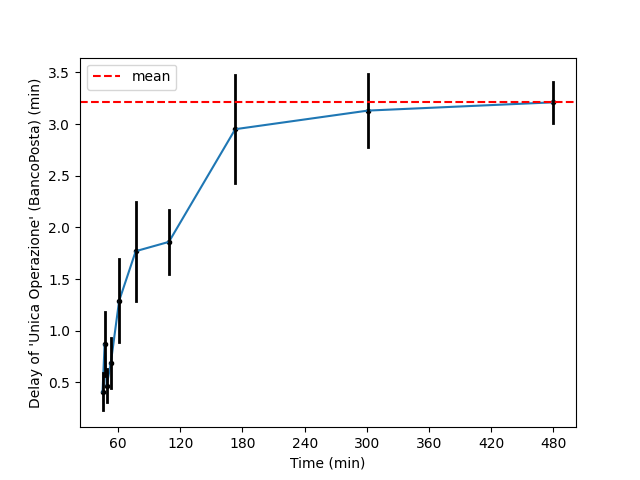
\includegraphics[width=\textwidth]{plots/day-from-empty-0}
\caption{\uo{} \textsl{BancoPosta}}    
\label{fig:esperimenti-simulazione-2a}
\end{subfigure}
\hfill    
\begin{subfigure}[b]{0.475\textwidth}  
\centering 
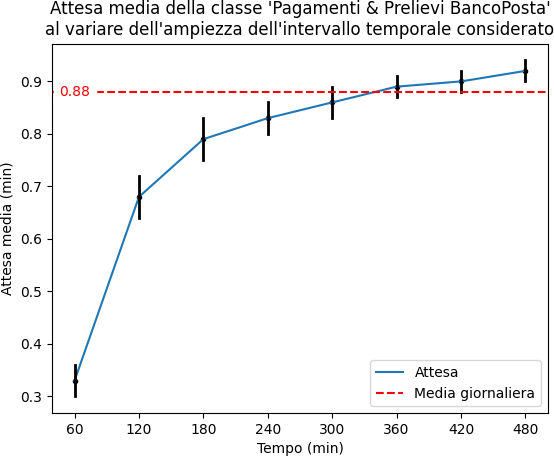
\includegraphics[width=\textwidth]{plots/day-from-empty-1}
\caption{\pp{} \textsl{BancoPosta}}
\label{fig:esperimenti-simulazione-2b} 
\end{subfigure}

\vskip\baselineskip

\begin{subfigure}[b]{0.475\textwidth}   
\centering 
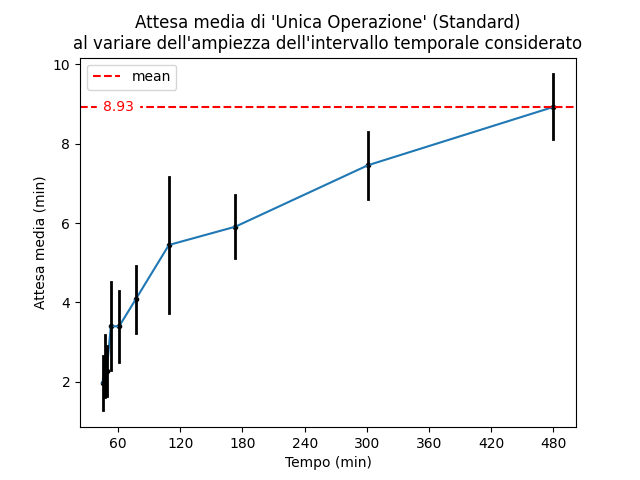
\includegraphics[width=\textwidth]{plots/day-from-empty-2}
\caption{\uo{} \textsl{Standard}}
\label{fig:esperimenti-simulazione-2c}
\end{subfigure}
\hfill
\begin{subfigure}[b]{0.475\textwidth}   
\centering 
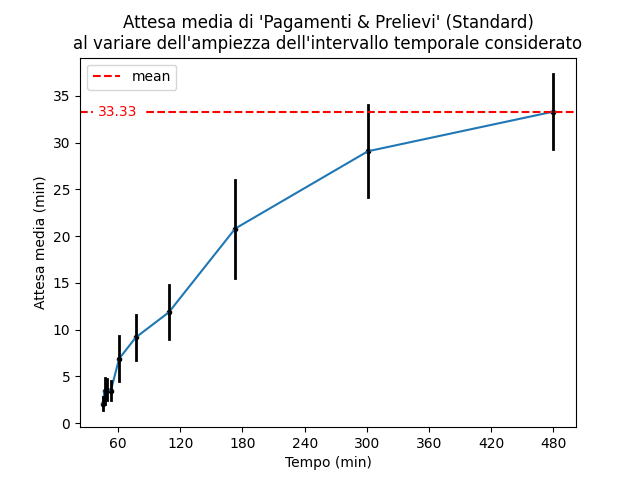
\includegraphics[width=\textwidth]{plots/day-from-empty-3}
\caption{\pp{} \textsl{Standard}}    
\label{fig:esperimenti-simulazione-2d}
\end{subfigure}

\vskip\baselineskip

\begin{subfigure}[b]{0.475\textwidth}   
\centering 
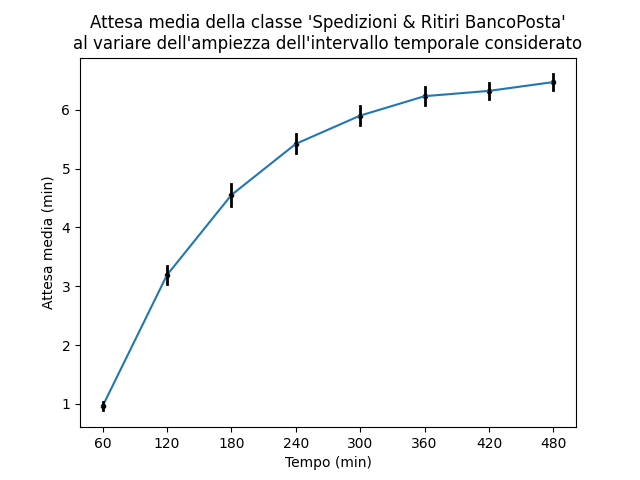
\includegraphics[width=\textwidth]{plots/day-from-empty-4}
\caption{\sr{} \textsl{BancoPosta}}    
\end{subfigure}
\hfill
\begin{subfigure}[b]{0.475\textwidth}   
\centering 
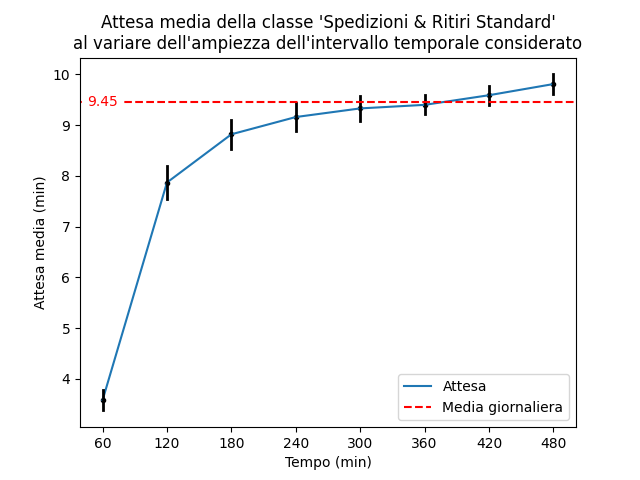
\includegraphics[width=\textwidth]{plots/day-from-empty-5}
\caption{\sr{} \textsl{Standard}}    
\end{subfigure}
\caption{Intervalli di confidenza al 95\% per l'attesa media (espressa in minuti) di ciascuna classe d'utenza, al variare dell'istante di campionamento}
\label{fig:esperimenti-simulazione-2}
\end{figure}

\captionsetup[figure]{justification=centering}
\begin{figure}[ht]
\centering
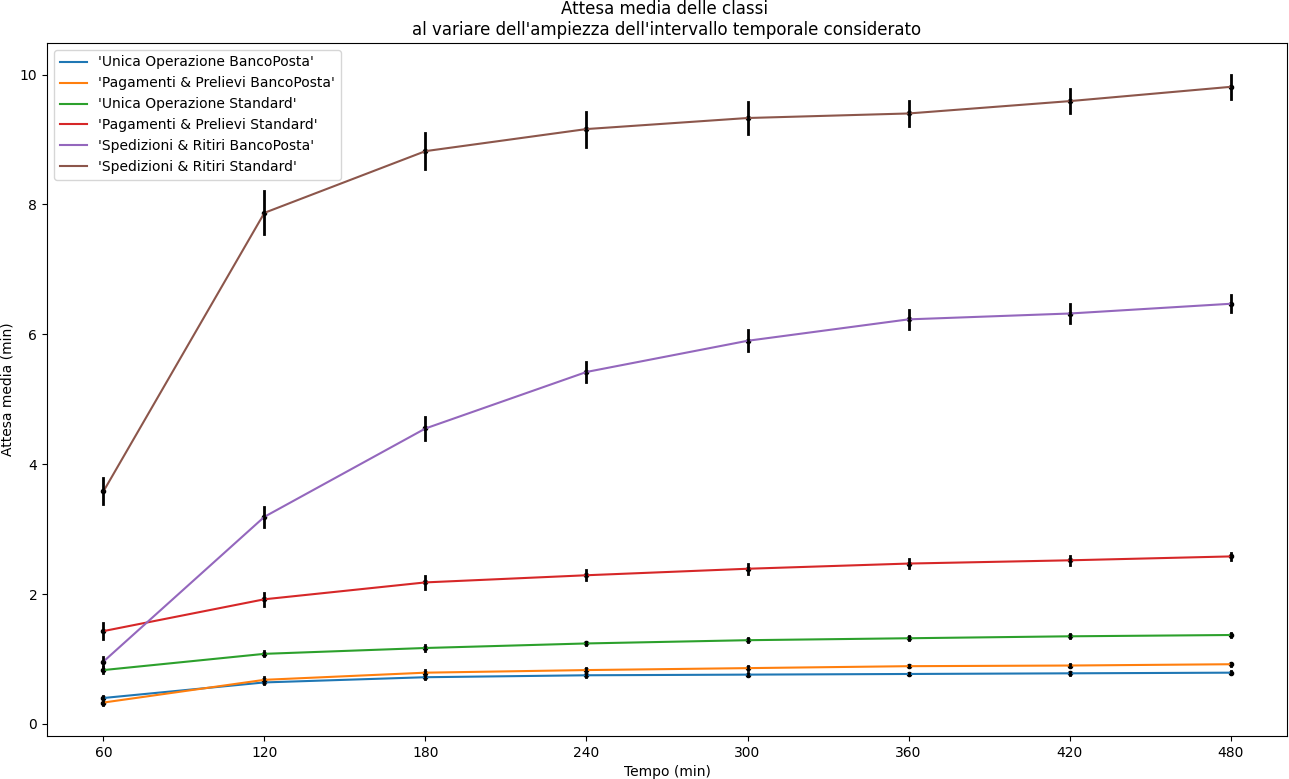
\includegraphics[width=\textwidth]{plots/day-from-empty-all}
\caption{Intervalli di confidenza al 95\% per l'attesa media (espressa in minuti) di tutte le classi d'utenza, al variare dell'istante di campionamento}
\label{fig:esperimenti-simulazione-3}
\end{figure}

\subsection*{Mancato raggiungimento dello stato stazionario}
\captionsetup[table]{justification=centering}
\begin{table}[ht]
\centering
{\tablecolors
\begin{tabular}{|c|c|c|c||c|c|c|c|}
\hline
$t$ & $\bar{d}_2$ & $s_2$ & $w$ & $t$ & $\bar{d}_2$ & $s_2$ & $w$ \\
\hline
60 & 0.846 & 2.827 & 0.06 & 540 & 1.374 & 1.263 & 0.02 \\
\hline
120 & 1.045 & 2.002 & 0.04 & 600 & 1.385 & 1.204 & 0.02 \\
\hline
180 & 1.167 & 1.791 & 0.04 & 660 & 1.392 & 1.147 & 0.02 \\
\hline
240 & 1.242 & 1.628 & 0.03 & 720 & 1.397 & 1.098 & 0.02 \\
\hline
300 & 1.289 & 1.528 & 0.03 & 780 & 1.405 & 1.059 & 0.02 \\
\hline
360 & 1.324 & 1.518 & 0.03 & 840 & 1.413 & 1.027 & 0.02 \\
\hline
420 & 1.348 & 1.407 & 0.03 & 900 & 1.418 & 0.996 & 0.02 \\
\hline
480 & 1.362 & 1.322 & 0.03 & 960 & 1.423 & 0.971 & 0.02 \\
\hline
\end{tabular}}
\caption{Istante di campionamento ($t$), media ($\bar{d}_c$), deviazione standard ($s_c$) e ampiezza dell'intervallo di confidenza al 95\% ($w$) per l'attesa (espressa in minuti) della classe d'utenza \uo{} \textsl{Standard}}
\label{table:esperimenti-simulazione-3}
\end{table}

\captionsetup[figure]{justification=centering}
\begin{figure}[ht!]
\centering
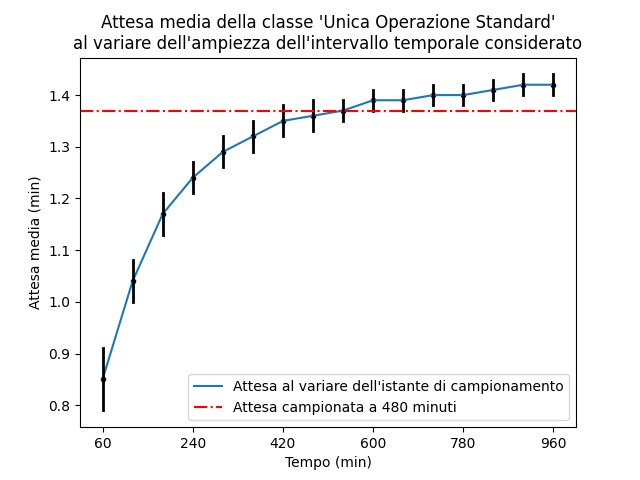
\includegraphics[width=0.8\textwidth]{plots/d2-no-stat}
\caption{Intervalli di confidenza al 95\% per l'attesa media (espressa in minuti) della classe d'utenza \uo{} \textsl{Standard}}
\label{fig:esperimenti-simulazione-4}
\end{figure}